\section{Ergebnisse}
\label{sec:ergebnisse}

\subsection{Experimentelles Setup}
Die in Abschnitt \ref{sec:methode} beschriebenen Trainings- und
Auswertungsbedingungen werden hier als bekannt vorausgesetzt. Im Folgenden
konzentrieren wir uns auf die präsentierten Resultate, deren Einordnung und die
relevanten Schlussfolgerungen für die Wahl von Architektur und Regularisierung.

\subsection{Quantitative Ergebnisse}
Die zusammenfassende Übersicht aller Validierungs- und Test-Accuracies ist in
Tabelle \ref{tab:results} im Anhang zu finden. Daraus ergibt sich klar ein
Leistungsgefälle: Modelle mit Batch-Normalisierung erreichen durchgängig höhere
Accuracy-Werte als vergleichbare Modelle ohne BatchNorm. Besonders hervorzuheben
ist das Modell \emph{BatchNorm\_Dense\_Pool\_Conv\_Net}, das mit einer
Validierungs-Accuracy von 85.8\% und einer Test-Accuracy von 84.2\% das beste
Ergebnis erzielt. Das Basismodell \emph{Base\_Net} liegt demgegenüber bei
57.9\% (Val) bzw. 59.6\% (Test).

Abbildung \ref{fig:compare_best_base} vergleicht den Trainingsverlauf des
besten Modells direkt mit dem \emph{Base\_Net}. Während das Basisnetz einen
gleichmäßigeren, weniger schwankenden Verlauf zeigt, erzielt das BatchNorm-Netz
ein deutlich höheres Leistungsniveau, geht aber mit stärkeren epochalen
Schwankungen einher. Diese Differenz spricht dafür, dass BatchNorm die
Optimierung beschleunigt und das erreichbare Endniveau anhebt, zugleich jedoch
die Kurven etwas volatiler macht.

\begin{figure}[H]
      \centering
      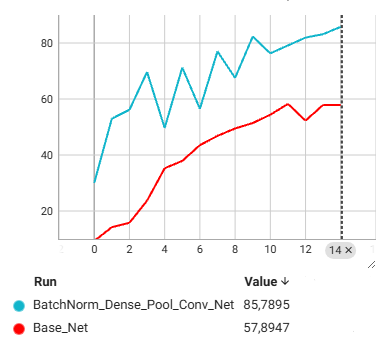
\includegraphics[width=0.85\linewidth]{figures/CompareBestBase.png}
      \caption{Vergleich der Validierungsverläufe von \emph{Base\_Net}
            (rot) und \emph{BatchNorm\_Dense\_Pool\_Conv\_Net} (blau). Das
            BatchNorm-Modell erreicht ein deutlich höheres Leistungsniveau, zeigt
            aber stärkere epochale Schwankungen als das stabilere Basismodell.}
      \label{fig:compare_best_base}
\end{figure}

In unseren Läufen war Overfitting allgemein wenig ausgeprägt: Trainings- und
Validierungsverläufe divergierten nicht stark, was auf sinnvolle
Regularisierung und die angewandten Augmentationsstrategien hindeutet.

\subsection{Konfusionsmatrix und klassenweise Analyse}
Die klassenweise Betrachtung der Fehlklassifikationen ergänzt die globalen
Accuracy-Werte: Die Konfusionsmatrix des besten Modells [\ref{fig:best_confusion}] ist nahezu diagonal und
zeigt nur noch wenige, konsistente Verwechslungen zwischen visuell ähnlichen
Klassen. Typische Fehlerpaare sind \emph{ferry\_terminal} mit
\emph{harbor}, \emph{overpass} mit \emph{intersection} sowie
\emph{sparse\_residential} mit \emph{dense\_residential}. Die Konfusionsmatrix
des schlechtesten Modells [\ref{fig:worst_confusion}] dagegen weist eine deutlich verwischtere Diagonale auf
und verteilt Fehlklassifikationen breiter über das Raster.

Aus dieser Analyse lässt sich ableiten, dass die verbleibenden Fehler größtenteils
auf inhärente visuelle Ähnlichkeiten zwischen bestimmten Klassen zurückzuführen
sind und weniger auf generelle Mängel der Trainingsprozedur.

\subsection{Interpretation und qualitative Beobachtungen}
Die Ergebnisse lassen sich folgendermaßen zusammenfassen: Insgesamt deuten die
Resultate darauf hin, dass Batch-Normalisierung die Modellleistung deutlich
verbessert; das beste BatchNorm-Modell (\emph{BatchNorm\_Dense\_Pool\_Conv\_Net})
erreicht 85.8\% (Val) bzw. 84.2\% (Test) und liegt damit weit über dem
\emph{Base\_Net}. Komplexere Varianten wie
\emph{BatchNorm\_Dense\_Pool\_Conv\_Dropout\_V2\_Net} (80.0\% Val,
77.2\% Test) zeigen hingegen keinen klaren zusätzlichen Nutzen im Verhältnis zu
ihrem erhöhten Ressourcenbedarf.

Dropout wirkt in unseren Experimenten primär als Varianz-Reduktor der Lernkurven
und kann unter Umständen die Konvergenz verlangsamen; seine konkrete Wirkung ist
aber architekturabhängig. Insgesamt legen die vorliegenden Kurven und
Konfusionsmatrizen nahe, dass die Wahl von BatchNorm in Kombination mit einer
ausreichenden, aber nicht übertriebenen Modellkomplexität den besten
Trade-off zwischen Leistung und Aufwand liefert.